\documentclass[pdftex,12pt,a4paper]{report}

\usepackage[portuguese,english]{babel}
\usepackage[T1]{fontenc} 
\usepackage[utf8]{inputenc}
\usepackage[pdftex]{graphicx}
\usepackage{minitoc}
\usepackage{hyperref}
\usepackage{indentfirst}
\usepackage[compact]{titlesec}
\usepackage{fancyhdr}
\usepackage{caption}
\usepackage{pgfplots}
\usepackage{pgfplotstable}
\usepackage{fixltx2e}
\usepackage{mathtools}
\usepackage{fancyhdr}
\usepackage{listings}
\usepackage{color}
\usepackage{sverb}
\usepackage[section]{placeins}

%Highlight
\newcommand{\shellcmd}[1]{\\\indent\indent\texttt{\footnotesize\# #1}\\}

\pagestyle{fancy}
\renewcommand*\thesection{\thechapter\arabic{section}}
\newcommand{\HRule}{\rule{\linewidth}{0.5mm}}
\begin{document}

\begin{titlepage}

\begin{center}


\includegraphics[width=0.15\textwidth]{./logo}\\[0.5cm]    

\textsc{\large Universidade de Aveiro \\[1cm]\large departamento de electrónica, telecomunicações e informática}\\[1cm]

\textsc{\large{47232}\large - Segurança \\[1cm]}

\HRule \\[0.5cm]
{ \huge \bfseries  IEDCS}\\[0.4cm]
{ \large \bfseries Identity Enabled Distribution Control System}\\[0.4cm]
\HRule \\[1cm]

\textsc{\small{8240 - MESTRADO INTEGRADO EM ENGENHARIA DE COMPUTADORES E TELEMÁTICA}}\\[1cm]

\begin{minipage}{0.4\textwidth}

\begin{flushleft} \large
\href{mailto:rafael.ferreira@ua.pt}{António Rafael da \\ Costa Ferreira }
 \small{\\NMec: 67405 | P4G1}
\end{flushleft}
\end{minipage}
\begin{minipage}{0.4\textwidth}

\begin{flushright} \large
\href{mailto:rodrigocunha@ua.pt}{Rodrigo Lopes \\ da Cunha}
\small{\\NMec: 67800 | P4G1}
\end{flushright}
\end{minipage}\\[1cm]

{\large Docente: João Paulo Silva Barraca   }\\[0.5cm]

\vfill

{\large Novembro de 2015 \\ 2015-2016}

\end{center}

\end{titlepage} %Titulo do Relatorio
\renewcommand{\headrulewidth}{0pt}

%Cabeçalhos de rodapé
\fancyhead{}
\fancyfoot{}
\lhead{IEDCS: Identity Enabled Distribution Control System}
\rhead{Seg. - 2015/2016}
\lfoot{\textit{P4G1} \\ Rafael Ferreira nmec: 67405 \\ Rodrigo Cunha nmec: 67800}
\rfoot{\thepage}

%Renomear Comandos
\renewcommand*\contentsname{Conteúdos}
\renewcommand*\figurename{Figura}
\renewcommand*\tablename{Tabela}

%Conteúdos, dar paragrafo
\tableofcontents
%Headers
\renewcommand{\headrulewidth}{0.15pt}
\renewcommand{\thechapter}{}


\clearpage

\section{Introdução}
% o que, porquê e o objetivo
O trabalho proposto para o projeto da unidade curricular de Segurança é um IEDCS: Identity Enabled Distribution Control System. Para o  efeito foi necessário implementar uma Ebook Webstore, um WebService e um Player de reprodução dos Ebooks em formato de texto.

O objetivo deste sistema é garantir a máxima e possível segurança do serviço, utilizando os conhecimentos adquiridos na unidade curricular de Segurança. Para isso são necessários vários processos como por exemplo, a utilização de certificados HTTPS, a cifragem de todo o material existente, derivação de chaves e registo de utilizadores.	

O relatório reflete todos os passos e decisões tomadas na criação do sistema, assim como uma análise ao que foi mostrado na primeira apresentação e decisões que se tomaram depois desta, tecnologias utilizadas, descrição dos vários processos existentes e conclusão.

\newpage
\section{Processos apresentados na 1ª apresentação}

\subsection{Processo de cifra do conteúdo do livro}
Na primeira apresentação foram concebidos dois processos que foram abandonados após a sua apresentação. O primeiro processo apresentado foi o “Book content cipher process”. Este pretendia fazer uso de cifras simétricas e assimétricas de forma a ser possível obter uma File Key que seria usada para cifrar o conteúdo do livro. Idealmente o conteúdo do livro seria cifrado com a chave privada do Player, depois cifrado com a chave pública do Device e finalmente seria feito sobre esses resultados uma cifra com o User Key e a File Key. O processo de cifra com o User Key e a File Key seriam repetidos n vezes, sendo o n obtido através do random2. Foi pensado também usar duas funções para derivar as keys, uma f1 que seria usada para derivar a User Key e uma f2 que seria usada para derivar a File Key.

A ideia de usar uma função de derivação da File Key e da User key é boa, e usando um número de iterações finita também. Isto permite que quem esteja a ouvir na rede tenha mais dificuldades em obter uma chave usando aquilo que conseguiu ouvir, pois teria de conhecer o processo usado pelos intervenientes para conseguir obter as chaves. Diga-se que também não seria difícil perceber o processo usado pelos dois intervenientes pois basta ao atacante usar o serviço e obter um Player e usando ferramentas próprias analisar o código.

A causa de ter-se abandonado este processo para cifrar o conteúdo do livro foi:

\begin{itemize}  
        \item É computacionalmente exigente cifrar com chaves assimétricas conteúdos grandes.
        \item Normalmente para evitar este esforço computacional faz-se uma assinatura sobre o resultado de uma função de síntese desse mesmo conteúdo do livro.
        \item As chaves simétricas são muito mais eficientes a nível computacional.
        \item As funções para derivar as chaves foram abandonadas em detrimento da PBKDF2 que efetua já as iterações idealizadas.
        \item Não é boa ideia usar as passwords dos utilizadores para cifrar o conteúdo do mesmo pois caso o utilizador mude a password ter-se-ia de derivar as chaves outra vez.
\pagebreak
                
\end{itemize}

\begin{figure}[!htb]
\center
 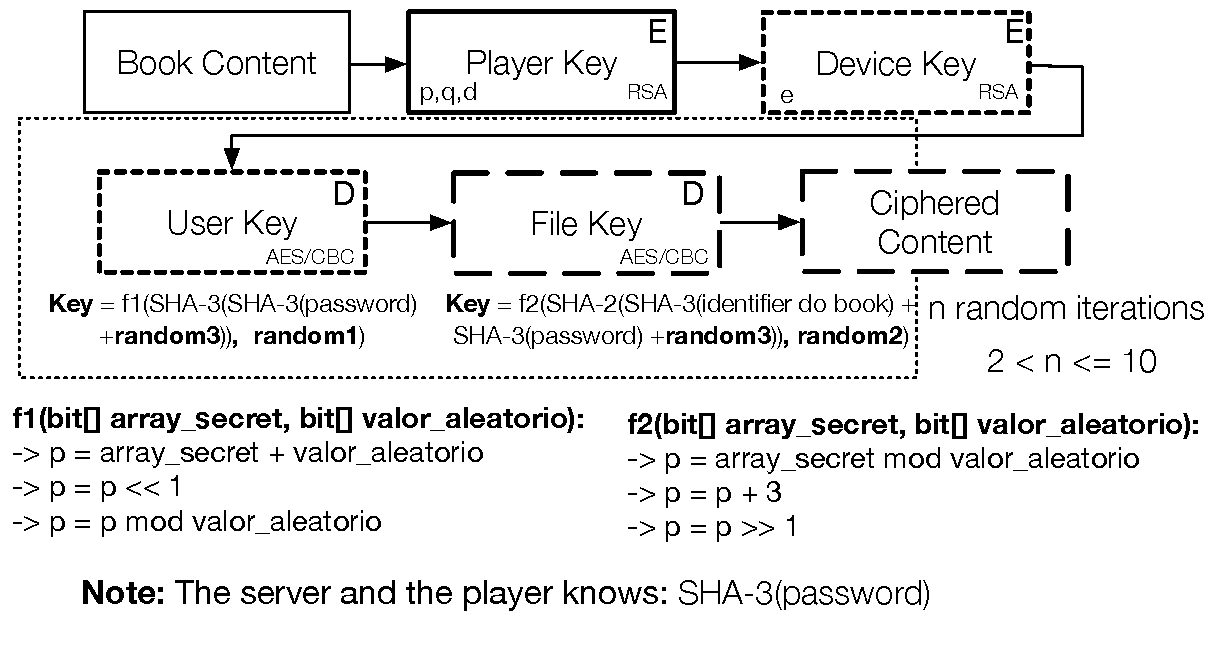
\includegraphics[width=135mm,scale=1]{filekey-initial-crypt.pdf}
 \caption{\\Processo de cifra usado na 1º apresentação}\label{fig:eer}
\end{figure}

\subsection{Processo de decifra do conteúdo do livro}
O processo de decifra foi desenhado para reverter o processo anunciado em cima. Sendo por isso nada mais do que fazer as operações inversas das realizadas no processo de cifra. As razões para que se tenha abandonado este processo de decifra são as mesmas enunciadas no processo de cifra.

O processo de “challenge” consistia no pedido do \textit{random1} e do \textit{random2} ao servidor, mas, isso não é suficiente para que o processo seja seguro, pois basta ao atacante conhecer o processo de cifra e decifra e intercetar os pedidos ao servidor do \textit{random1} e do \textit{random2}. Para o Player também seria fácil decifrar sem necessitar da cooperação do servidor, pois, bastava que cooperasse uma primeira vez.

\begin{figure}[!htb]
\center
 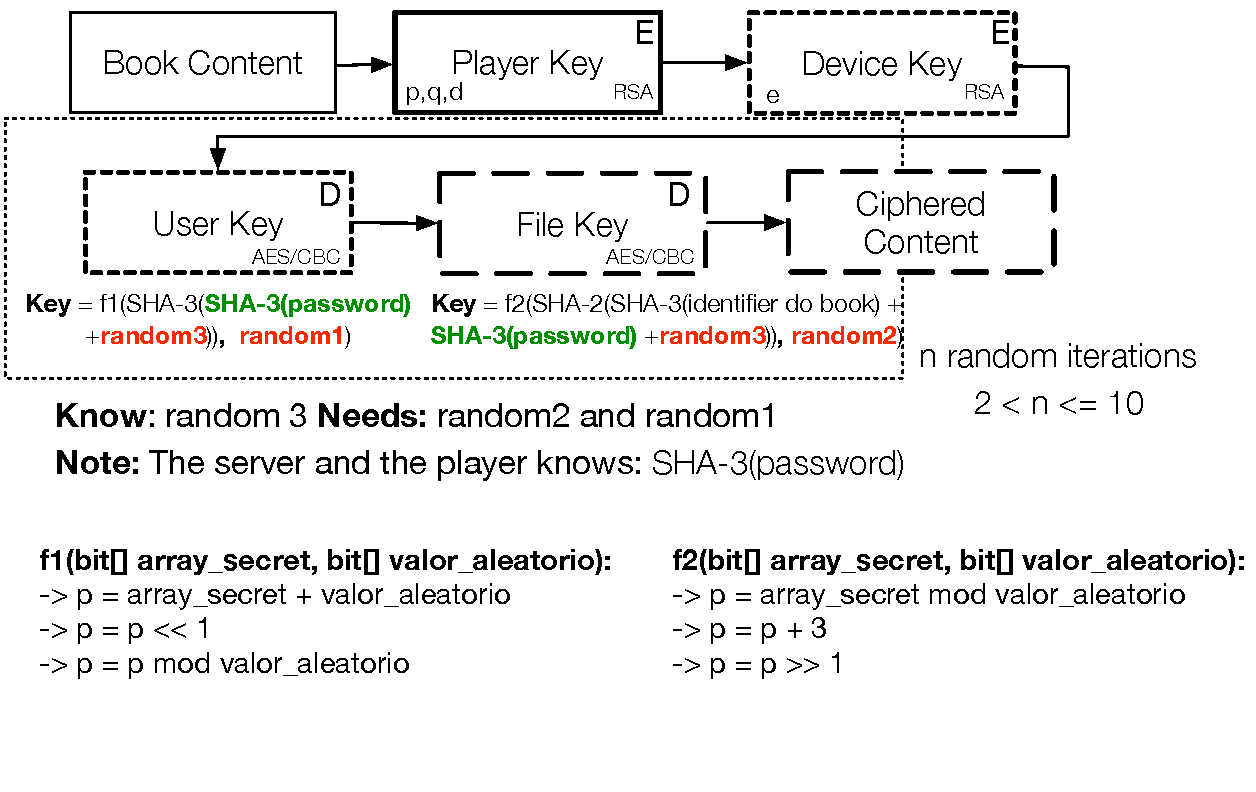
\includegraphics[width=135mm,scale=1]{filekey-initial-decrypt.pdf}
 \caption{\\Processo de decifra usado na 1º apresentação}\label{fig:eer}
\end{figure}

\section{Alterações efetuadas em relação à 1ª apresentação}

No seguimento da primeira apresentação procedeu-se a muitas alterações no modo como o processo de cifra e decifra do conteúdo de um livro seria efetuado.	

\subsection{Processo de cifra do conteúdo do livro}

\begin{figure}[!htb]
\center
 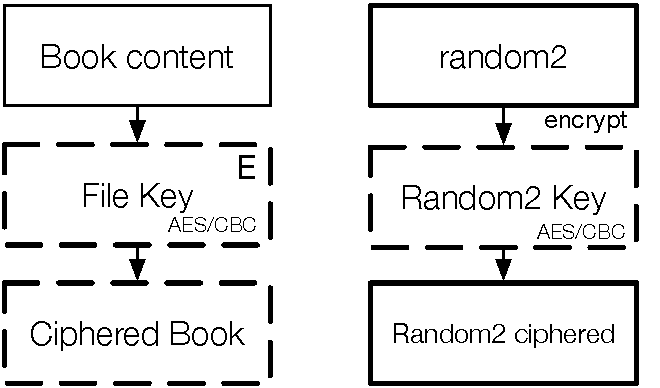
\includegraphics[width=50mm,scale=1]{book-cipher-process.pdf}
 \caption{\\Processo de cifra de um livro}\label{fig:eer}
\end{figure}

Neste novo processo, o servidor cifra um valor aleatório, designado por Random2, com uma chave Random2 Key, calculada através da seguinte forma:

\begin{center}
	\textbf{Random2 Key = PBKDF2(username + “jnpc” + book.identifier, book.identifier, 1000)}
\end{center}

Esta key é partilhada pelo servidor e pelo cliente, pois ambos conhecem a forma de como ela é calculada, não sendo preciso enviar a mesma. Apenas o conteúdo de Random2 cifrado é enviado para o cliente. 
O valor Random2 foi criado, para que através dele tanto o servidor como o cliente possam obter a File Key que será utilizada para cifrar o conteúdo de um livro que não poderá ser guardada do lado do cliente e poderá ser reutilizada para um mesmo utilizador noutro Player ou noutro Device.

\begin{figure}[!htb]
\center
 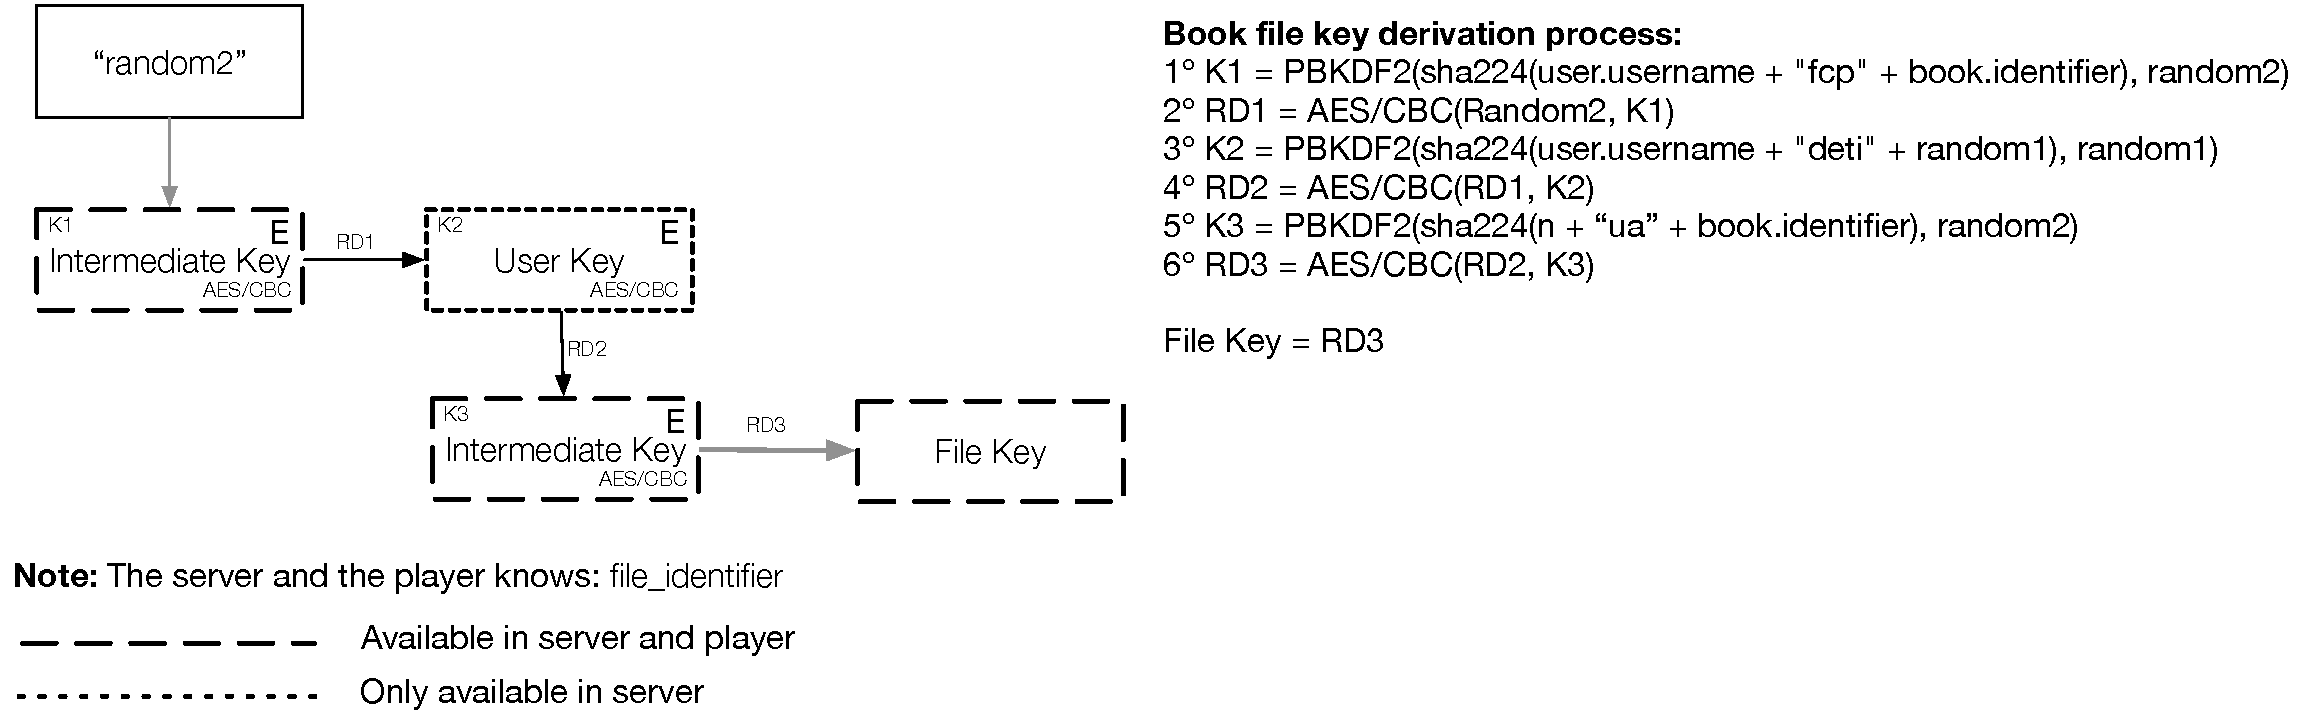
\includegraphics[width=150mm,scale=1]{file-key-generation.pdf}
 \caption{\\Processo de derivação da File Key}
 \label{fig:processo_de_derivacao_file_key}
\end{figure}

Para derivar a File Key, como se pode ver na figura \ref{fig:processo_de_derivacao_file_key}, o Random2 é cifrado com uma chave K1, que é calculada através do SHA-224 do username, de um texto (“fcp”) e do identificador do livro. Este SHA é a password e o Random2 o texto, aplicando-se assim a função PBKDF2 (recomendado na apresentação), com o valor por defeito de 1000 iterações, obtendo-se assim a chave pretendida, K1. O cálculo desta chave K1 é possível de ser efetuado tanto do lado do servidor como do cliente.

Posto isto, o resultado obtido da cifra de Random2 com a chave K1, RD1, vai ser cifrado com uma nova chave K2, sendo esta apenas calculada pelo servidor. Esta é calculada praticamente como a K1, sendo diferente por no SHA-224 utilizar um outro texto (“deti”) e um \textit{random1}, em vez de \textit{random2}, apenas disponível no servidor, em vez de usar o identificador do livro. Aplica-se igualmente a função PBKDF2, com o SHA como password e o \textit{random1} como texto, de forma a obter K2 para se poder cifrar o valor de RD1.

Numa última fase deste processo de derivação da File Key, é calculada ainda uma terceira chave, K3, com o mesmo processo das outras chaves K1 e K2, sendo nesta última utilizado no calculo do SHA um valor n, que corresponde a:

\begin{center}
	\textbf{n = (soma de todos os digitos de random2) \% 10}
\end{center}

Juntamente com o valor n, utiliza-se o identificador do livro e um texto “ua”. Através deste SHA e do random2 que atuam respetivamente como password e salt, aplica-se uma função PBKDF2 para obter K3.

Por último através da cifra de RD2 (valor obtido da cifra de \textit{random1} com a chave K2) com a chave K3 obtida, obtém-se a File Key, que será utilizada para cifrar o conteúdo do livro e desta forma este conteúdo cifrado será enviado para o cliente.

\subsection{Cifra simétrica e modo}

Todo o processo de cifra e decifra de um livro e de um random2, foi efetuado através da cifra simétrica por blocos AES com o modo de cifra CBC.

Foi escolhida a cifra simétrica AES, pois cifra por blocos e garante maior rapidez tanto no processo de cifra como de decifra.
	
O modo de cifra CBC foi selecionado devido à existência de confusão, introduzida por um IV no inicio do processo de cifra e decifra. Cada bloco cifrado funciona como realimentação para o bloco seguinte, exceto no inicial, onde é utilizado o IV. Isto permite ter acesso aleatório uniforme apenas na decifra, que é o pretendido para o método de paginação, sendo então possível decifrar o bloco que se deseja, sem ter de processar os anteriores. 

\subsection{Visualização de um livro}
Na primeira vez que um utilizador solicita a visualização de um livro é gerado o primeiro Random2 e Random1 que vai ser único para determinado utilizador e livro que tenha adquirido o livro. Estes valores aleatório são guardados na base de dados cifrados com uma chave que depende do utilizador e do livro.

Todos os Initialization Vectors são também guardados na base de dados com o mesmo processo.

Os Random2, Random1 e Initialization Vectors passam todos por um processo de cifra antes de serem guardados na base de dados. Este processo consiste em:

\begin{itemize}
\item Gerar um \textit{identifier}, através de um SHA-224 composto por um alias (nome pelo qual se quer identificar o conteúdo, por exemplo “random2”), username e identificador do livro.
\item Gerar um valor que será a password na função PBKDF2, através de um SHA-224, composto pelo username, email e último nome.
\item Depois de gerados os dois valores acima descritos, recorre-se a uma função PBKDF2, onde o salt é o \textit{identifier}. Esta função terá um número de 1000 iterações por defeito.
\item Posto isto, o conteúdo que se deseja guardar na base de dados é cifrado com a chave gerada acima, ficando assim salvaguardado com alguma segurança.
\end{itemize}

\subsection{Processo de decifra do conteúdo do livro}

\begin{figure}[!htb]
\center
 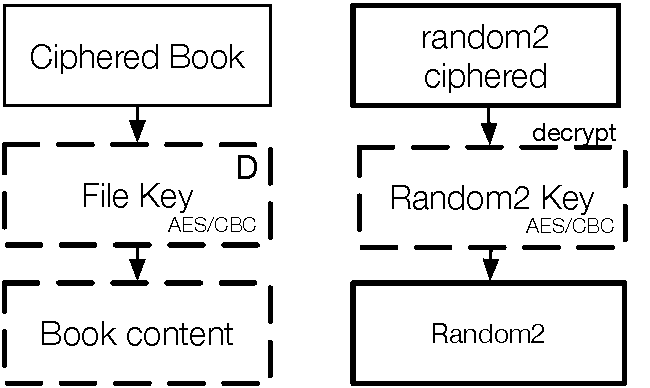
\includegraphics[width=50mm,scale=1]{book-decipher-process.pdf}
 \caption{\\ Processo de decifra de um livro}
 \label{fig:decifra_livro}
\end{figure}

Tal como no processo de cifra de um livro, a Random2 Key é calculada, mas desta vez no lado do cliente para este conseguir decifrar o random2 que recebeu cifrado, obtendo assim o valor original que vai ser utilizado para o cálculo da File Key usando também um processo de challenge.

\begin{figure}[!htb]
\center
 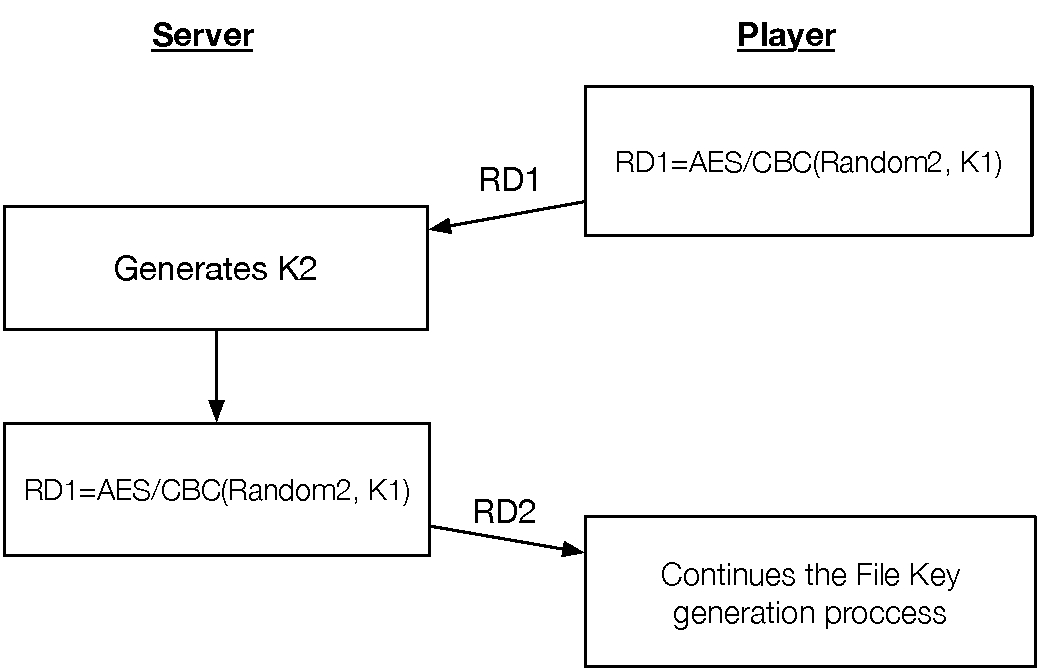
\includegraphics[width=80mm,scale=1]{challengefilekey.pdf}
 \caption{\\Challenge entre Player e Servidor na derivação da File Key}
 \label{fig:challange_player_server}
\end{figure}

O processo de derivação da File Key no lado do servidor e do cliente é feito da mesma maneira, apenas mudando, que quando o Player está a gerar a File Key, precisa de questionar o servidor (figura \ref{fig:challange_player_server}), pois ele é o único capaz de calcular o valor de RD2, obtido através da cifra de RD1 (cifra de Random2 com K1) com uma chave K2 calculada com um random1 que só o servidor conhece (figura \ref{fig:decifra_livro}). 

Este "challenge", que é um processo de pergunta e resposta, em que a pergunta tem de vir bem formulada, consiste na pergunta que o Cliente faz ao servidor, como já mencionado e na resposta, com o valor que calculou, para que o cliente prossiga o processo de derivação da File Key. 

A pergunta colocada ao servidor tem de ter um tamanho esperado e tem de ser colocada em Base64. Como a pergunta é em Base64 espera-se que a pergunta tenha um valor de 108 caracteres. 

O resultado da cifra de RD1 com AES/CBC tem 64 bytes, resultante de o random 2 ter 56 bytes (mais o padding ficam 4 blocos de 16 bytes cada). Com o IV soma-se 16 bytes. Tem-se então, 80 bytes a enviar para o servidor em Base64, sendo isto 640 bits. Como cada caracter é usado para representar 6 bits, mas como 640 não é múltiplo de 6 é preciso adicionar padding, neste caso, terá de ser adicionado 2 bits para ser múltiplo de 6 bits. Sendo assim 642 resulta em 107 caracteres, como apenas adicionou-se 2 bits apenas será necessário adicionar um '=' no final, resultando em 108 caracteres.

A resposta dada pelo servidor não é verificada se é a correta ou não pois isso poderia resultar em pedidos mal intencionados só para saber qual seria a resposta correta, e por consequência qual seria o valor de entrada correto para aquele livro e utilizador, resultando numa fraqueza no processo de cifra/ decifra.

Após este processo de derivação da File Key o Player decifra o conteúdo cifrado do livro de forma a obter o conteúdo original do mesmo, podendo agora apresenta-lo ao utilizador.

\newpage
\subsubsection{Paginação}

\begin{figure}[!htb]
\center
 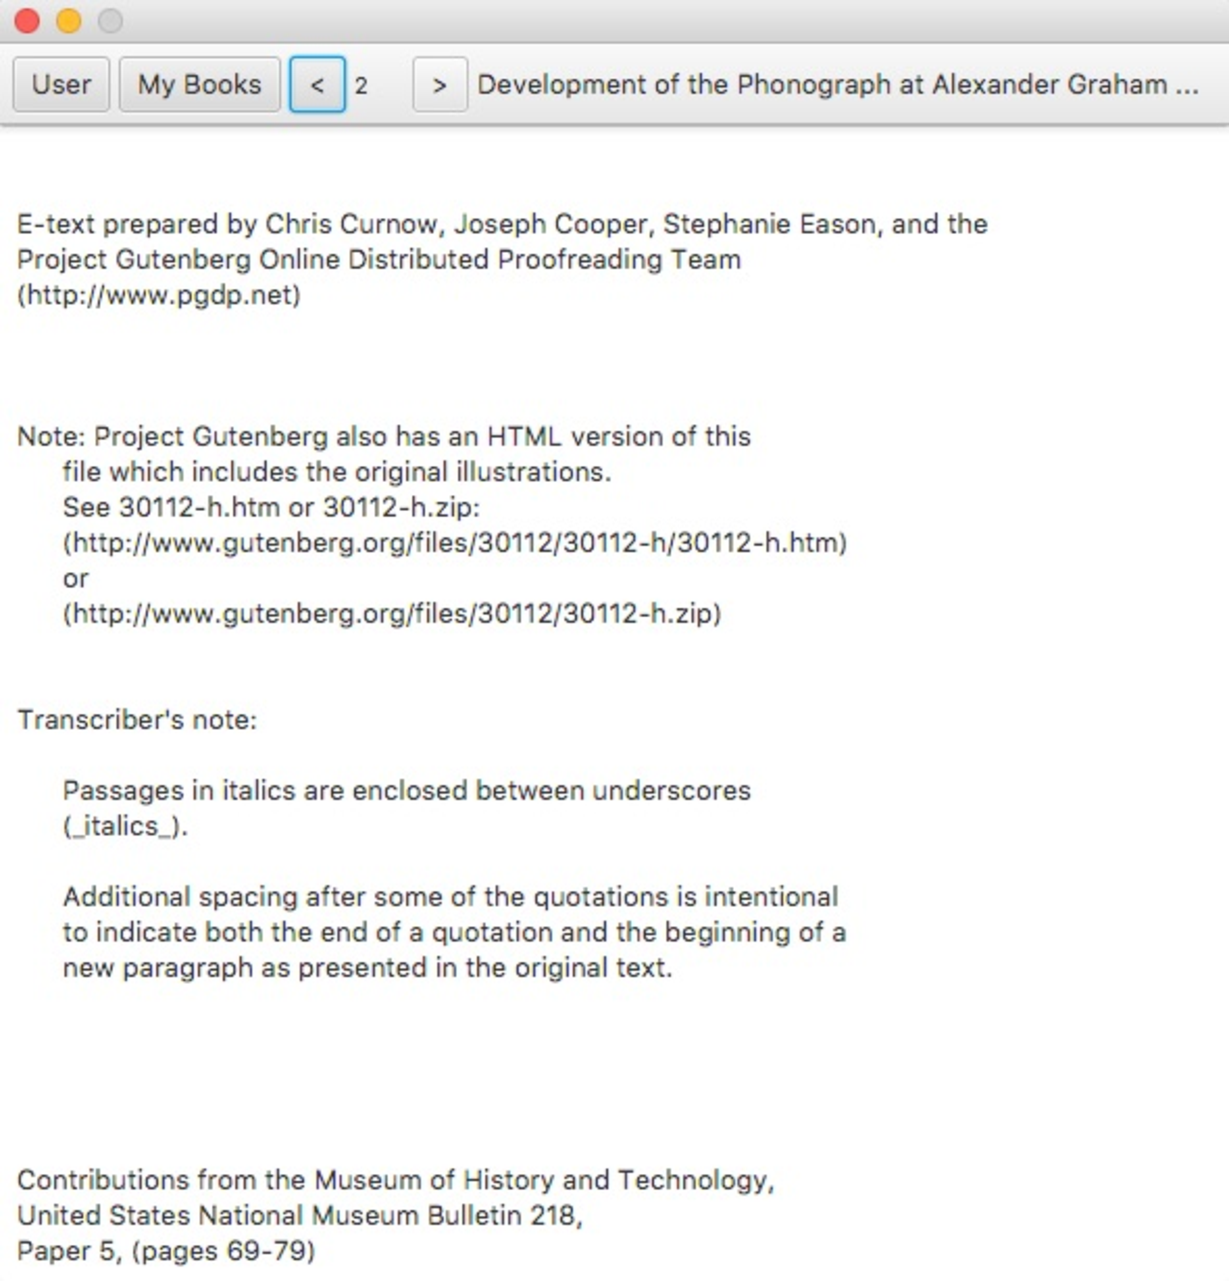
\includegraphics[width=80mm,scale=1]{Book_page.pdf}
 \caption{\\Paginação ajustada à janela}
 \label{fig:eer}
\end{figure}

A paginação foi feita de acordo com o tamanho da janela do Player de modo ao número de linhas ser igual a 31. Caso o último bloco a ser decifrado possua mais que uma linha, é apenas escrita a primeira linha desse bloco, sendo o resto do texto apresentado no início página seguinte.

Convém contudo realçar que a decifra do conteúdo é feita página a página, usando o acesso aleatório do modo CBC, e  a cada página apresentada ao utilizador são calculadas todas as chaves necessárias e é efetuado o challenge ao servidor.

\section{Tecnologias usadas}

As tecnologias usadas no desenvolvimento do IEDCS Server, foram: Django + Python e AngularJS + JS. O Django dá a possibilidade de usar proteção contra \href{https://docs.djangoproject.com/en/1.8/ref/csrf/}{CSRF} usando um token e um middleware que obriga que o cliente envie este token sempre que faz um pedido para a aplicação.  

O Angular.JS já tem suporte para enviar o CSRF token, sempre que recebe um \textit{Set-Cookie CSRFToken = XXX} na resposta do servidor, irá gravar esse csrf token num cookie no browser do utilizador e irá enviar sempre que for feito um pedido.

Já o Player foi feito usando Java e JavaFX. No java teve-se de usar uma biblioteca para fazer os pedidos HTTP e HTTPS exterior, neste caso usou-se a org.apache.http. Esta biblioteca não tem suporte para uso de um CSRF de forma correta, por isso, teve-se de implementar uma classe (Requests.java) que gerisse uma ligação HTTP e guardasse o seu estado de sessão. Nesta classe enviou-se um X-CSRFToken no Header do pedido.

No servidor, também teve-se a proteção contra SQL Injection e XSS ataques pois fez-se uso dos métodos disponibilizados pelo Django para manipulação de modelos da base de dados. Já o AngularJS não permite que seja injetado código JS nem HTML sem intenção do programador da aplicação.

Como se usou Python e Java já se teve proteção contra buffer overflows e mesmo assim teve-se cuidado para não fazer implementações que comprometessem o estado tanto do servidor como do player, como por exemplo, uma saída inesperada devido a um erro.

\section{Casos de utilização}

\subsection{Registo de um utilizador}

Um registo de um utilizador é feito na página web disponibilizada pelo IEDCS. Ao gravar na base de dados a password é gravada com um segundo PBKDF2 e SHA256, o que torna computacionalmente trabalhoso obter as passwords dos utilizadores caso a base de dados seja exposta. Ao fazer login, tanto no Player como na interface Web é aplicado PBKDF2 com HMAC e SHA1 para caso o HTTPS seja comprometido, as passwords não sejam enviadas em claro pela rede ou  caso se esteja a usar HTTP.

\begin{center}
	\textbf{Password = PBKDF2(Password, Password, 500)}
\end{center}

Não existe nenhuma criação da chamada UserKey, esta no entanto, é gerada para cada livro por cada utilizador quando ele solicita pela primeira vez a leitura do mesmo. Optou-se por fazer um UserKey por Livro para dificultar ainda mais a tarefa a quem tente comprometer o sistema de IEDCS.

\begin{figure}[!htb]
\center
 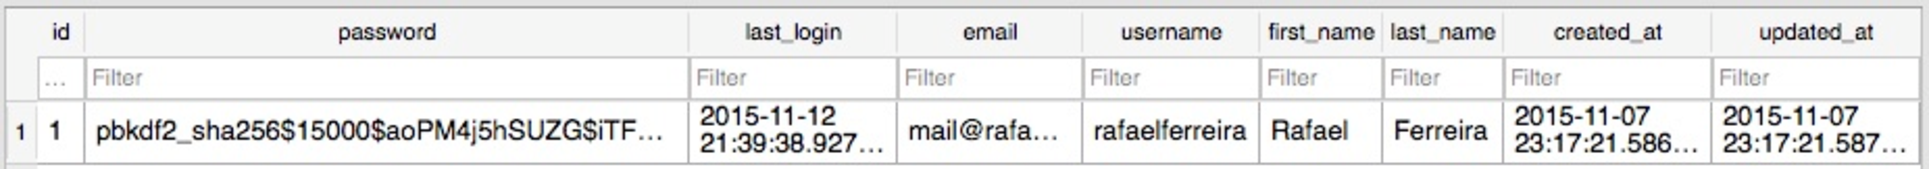
\includegraphics[width=150mm,scale=1]{pbkdf2_saved.pdf}
 \caption{\\Password guardada com PBKDF2 e SHA256}
 \label{fig:eer}
\end{figure}

\subsection{Registo de um device}
Quando um player é utilizado pela primeira vez num determinado device, no momento do login de um utilizador, o Device é registado na base de dados com os seguintes parâmetros:

\begin{itemize}
\item Identificador único
\item Modelo de CPU e PC
\item IP
\item País
\item Hora
\item Host name
\item Chave pública do Device
\end{itemize}

	No Player é usado a biblioteca sigar para obter os dados do device. O País é obtido no servidor através do IP recebido pelo mesmo.
	A cada utilizador também são associados os vários devices por onde já se conectou ao servidor.
	Caso no momento do login, o device já exista na base de dados, este é atualizado com os novos dados recebidos, tal como a hora, IP, entre outros já especificados.

\subsection{Aquisição de um livro}

No momento de aquisição do livro não há nenhuma cifra, apenas um registo na base de dados que o utilizador adquiriu um livro.

\subsection{Restrições na visualização de um livro}

\begin{figure}[!htb]
\center
 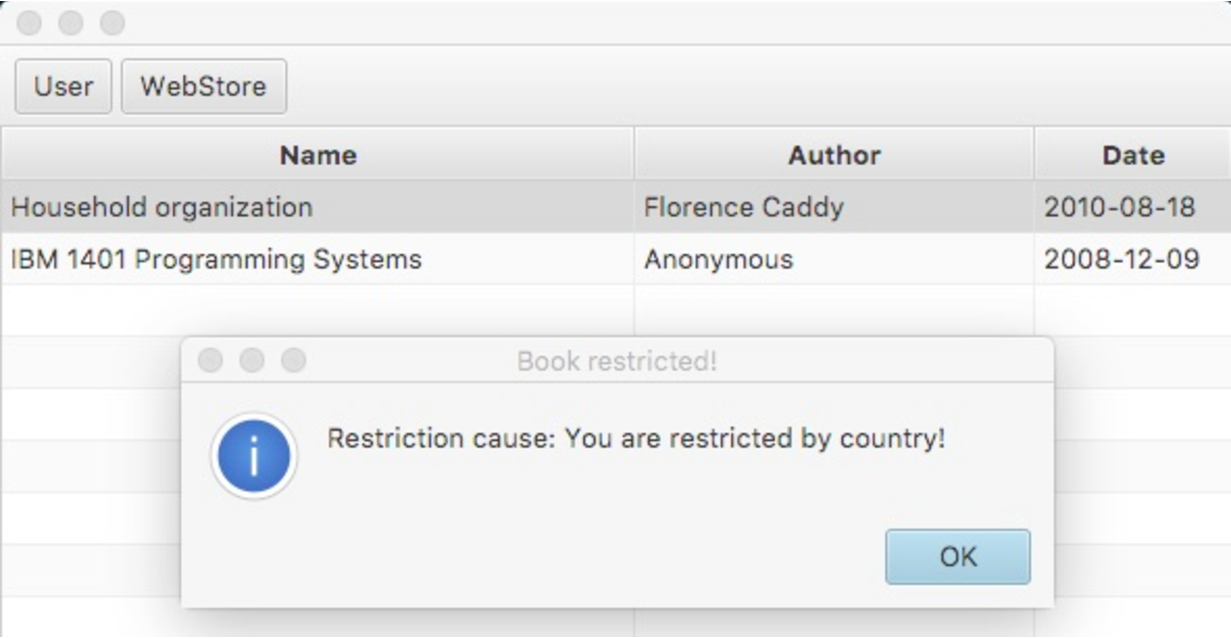
\includegraphics[width=100mm,scale=1]{country_restriction.pdf}
 \caption{\\Restrição apresentada tendo em conta o país do utilizador}
 \label{fig:eer}
\end{figure}

Para a visualização de um livro criaram-se dois tipos de restrições, por país e por hora de utilização.

Isto permite que os conteúdos não possam ser acedidos a qualquer momento e em qualquer lado caso existam restrições nesse livro.

\subsubsection{Gestão de restrições}

Para ser mais simples gerir as restrições por parte do administrador do sistema foi criada uma interface de linha de comandos com várias possibilidades. 
Para adicionar uma restrição a um livro:
\shellcmd{python manage.py restriction add restrict{\_}book book{\_}identifier \linebreak restriction{\_}name}
\linebreak
Para adicionar uma nova restrição no sistema:
\shellcmd{python manage.py restriction add restriction restriction{\_}name\linebreak restrictionFunction cause}
Para remover uma restrição a um livro:
\shellcmd{python manage.py restriction rm restrict{\_}book book{\_}identifier\linebreak restriction{\_}name}
Para listar os livros disponíveis:
\shellcmd{python manage.py restriction list books}

\section{Instalação}

Para uso e instalação do sistema, criou-se uma pasta /installation que tem um ficheiro \textit{Vagrantfile} que permite criar um servidor ubuntu trusty 64bits que cria uma pasta partilhada em /var/www que irá servir para lançar o servidor IEDCS com recurso ao Apache2. O ficheiro \textit{server-bootstrap.sh} servirá para instalar todas as bibliotecas necessárias, todos os pacotes do python, a configuração do Apache2 para o site que está no ficheiro \textit{iedcs.rafaelferreira.pt.conf} e \textit{default-ssl.conf}, também para instalar os certificados necessários para o HTTPS nas pastas usadas para esse efeito e para criar a base de dados com os livros e restrições exemplo.
	
O ficheiro \textit{iedcs.rafaelferreira.pt.conf} serve apenas para redirecionar todos os pedidos HTTP para HTTPS. O ficheiro \textit{default-ssl.conf} tem todas as configurações necessárias para o uso de HTTPS e para usar o modWSGI do Apache2 para o Django.

Criou-se um package de settings para o Django para ter definições de development e outras de servidor. Usando o hostname do servidor sabe-se em que modo deve estar, sendo assim nesse servidor iniciado com Vagrant o servidor estará em modo produção, ou seja, não irá lançar output de debug para o utilizador.

O \textit{install{\_}cert.sh} é usado para criar uma keystore que será usada pelo Java para armazenar os certificados em que ele confia ao usar HTTPS.	
	
Para usar o servidor, além de ter o \href{https://www.vagrantup.com/downloads.html}{Vagrant} intalado, é apenas necessário fazer:
\shellcmd{vagrant up}

A password caso seja pedida é sempre vagrant e para aceder à máquina é apenas necessário fazer: \shellcmd{vagrant ssh}

O site pode ser acessível em: \url{https://iedcs.rafaelferreira.pt/}

Para fazer download do Player apenas é preciso registar na webstore e depois clicar em "Player" que será feito o download do Player. A implementação do Player está apenas disponível para Mac OS X, com uma aplicaçãnative application  tendo como base uma aplicação JavaFX. Testado com o java version "1.8.0{\_}60".

\section{HTTPS}
Para criar um certificado criou-se uma chave privada RSA com:

\textit{openssl req -new -newkey rsa:2048 -nodes -keyout server.key -out server.csr}

\textbf{output:} /installation/ssl/generating.txt

O certificado foi depois emitido usando a \href{https://www.instantssl.com/free-ssl-certificate.html}{Free SSL}.

Como foi criado um domínio que aponta para o endereço \textit{192.168.33.10} que é o endereço local do servidor IEDCS inicializado pelo Vagrant.

\section{Problemas identificados na primeira entrega}

Nesta primeira entrega, identificaram-se alguns problemas, nomeadamente no corrompimento do HTTPS, através da troca da keystore onde são guardados os certificados confiáveis, podendo assim injetar todos os certificados que se deseja de forma a que seja possível intercetar as comunicações entre o servidor e o Player. Para isso sabe-se que o utilizador pode descompilar o código do Player, analisar o processo de cifra e o código. Com isto ele poderá descobrir que se usou um ficheiro cacerts.keystore para o Java confiar apenas no certificado usado, pode então modificar essa keystore e o cliente ao fazer download pode ser-lhe dada uma versão corrompida, mas sem estar corrompida no código, apenas no cacerts.keystore. Se estiver presente outro certificado que o atacante domine, ele pode intercetar as comunicações HTTPS e aceder às comunicações que estão a ser trocadas entre a vítima que está a usar o Player e o Servidor e assim, pode, obter o Random2 e derivar o n (este é enviado inicialmente num Header), o book identifier e o rd2 que é enviado pelo servidor no pedido de challenge ao cliente. O texto “ua” é possível de ser obtido descompilando o código. Posto isto, ele pode cifrar com AES e obter a file key. Com isto, consegue-se decifrar o livro cifrado.

Outra possibilidade seria um atacante/cliente que usasse ferramentas de análise de memória para obter o livro cifrado, e todas as outras variáveis que estão expostas em Runtime.

\subsection{Soluções}

\begin{itemize}
\item Assinar o Player com uma chave assimétrica assim como o ficheiro cacerts.keystore.
\item Autenticando ambas as entidades no momento em que é negociada o HTTPS entre o cliente e o servidor (2º parte do trabalho).
\item Sessão para a file key usada ser sempre diferente tendo em conta a sessão, proibindo a reutilização da file key em vários devices e players.
\item Cifra por página, ou seja, a paginação ser realizada no lado do servidor.
\end{itemize}

\newpage

\section{Segunda entrega, síntese de melhorias}

um género de introdução para a segunda entrega do trabalho <====

\section{Pequenas melhorias implementadas}

\subsection{New Secret Key}
Foram tidas em conta algumas considerações sobre o servidor Django. Muitas aplicações Django mantêm a "Secret Key" \footnote{\label{url1} \url{https://docs.djangoproject.com/en/1.9/ref/settings/\#secret-key}} a inicial que vem com outras instalações \footnote{\label{url1} \url{http://exfiltrated.com/research-Instagram-RCE.php}} da mesma framework, no entanto, para evitar algum problema, decidiu-se gerar uma nova chave privada para este projeto. 

\subsection{Django Rest Framework}
A DRF\footnote{\label{url1} \url{http://www.django-rest-framework.org/}} tem uma "browsable API"\footnote{\label{url1} \url{http://www.django-rest-framework.org/topics/browsable-api/}} que é usada para o utilizador que pretender  usar a API poder procurar, no entanto expor dessa forma endpoints não é aconselhável, por isso mesmo, foi retirado.


\subsection{Melhoria do Debug do Player}
Para o Player tinha-se desenvolvido uma interface para que quando a aplicação falha-se fosse possível fazer debug rapidamente do que se tinha passado, no entanto, tinham ficado falhas para o modo produção, sendo uma delas que em alguns casos era exposto para o utilizador os dados recebidos nos endpoints, sendo isto não aconselhável, melhorou-se a forma como é gerido o debug e o modo produção no Player. Sendo esta melhoria não muito importante, não se irá entrar em detalhes sobre a sua implementação.

\subsection{Copy/ Paste da janela do Player}
ALGO


\section{Confinamento}
Foram realizadas várias tentativas para fazer o confinamento da aplicação e limitar ao máximo o que a aplicação poderia fazer caso fosse comprometida e executasse código malicioso. Para isso, inicialmente, realizaram-se várias tentativas para implementar uma solução com \textit{chroot} e para a solução final usou-se Docker.

\subsection{Chroot with Apache}
O mod\_wsg\footnote{\label{url1} \url{https://code.google.com/p/modwsgi/}} na versão 0300\footnote{\label{url1} \url{https://code.google.com/p/modwsgi/wiki/ChangesInVersion0300}} anunciou a implementação de uma diretiva que permitia fazer o chroot de um \textit{WSGIProcess}. No entanto, esta funcionalidade está muito pouco documentada \footnote{\label{url1} \url{https://groups.google.com/d/msg/modwsgi/sOrtcm7JV50/YmriFHUmHI8J}}.

\begin{figure}[!htb]
\center
 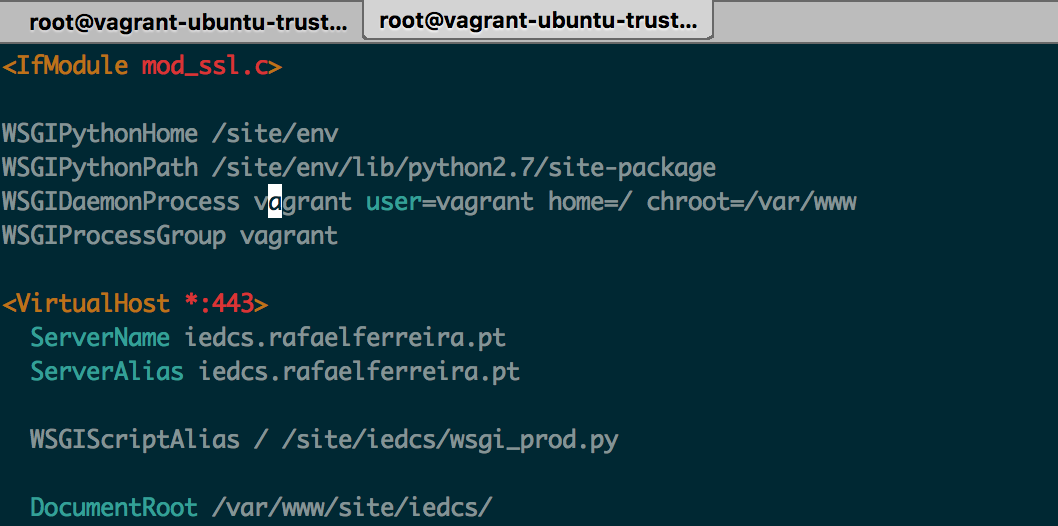
\includegraphics[width=100mm,scale=1]{apache_chroot_config.png}
 \caption{\\Parte da implementação do chroot}
 \label{fig:apache_chroot_config}
\end{figure}

No entanto, tentou-se a implementação, representada na figura \ref{fig:apache_chroot_config}, usando esta diretiva, os resultados obtidos usando a configuração, estão apresentados na figura ~ 

\begin{figure}[!htb]
\center
 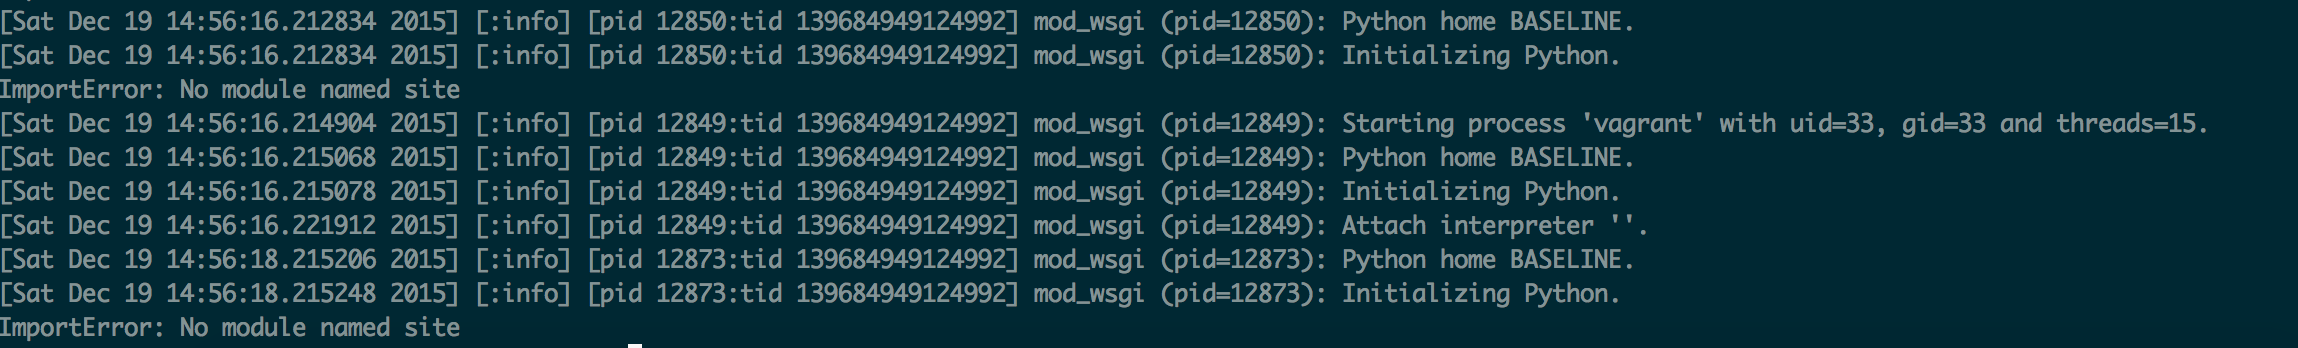
\includegraphics[width=100mm,scale=1]{import_error.png}
 \caption{\\Import Error: No module named site}
 \label{fig:import_Error}
\end{figure}

Com isto, foi abandonada a implementação de chroot com o apache para impedir que o python executa-se código de forma maliciosa e procurou-se outra solução.

\newpage
\subsection{Docker}
Para obter resultados semelhantes a um chroot pensou-se em usar o Docker. No entanto não se pode pensar só em usar Docker, teve-se de pensar numa arquitetura para o servidor e o contentor docker. Para isso, a principal preocupação, foi em ter as chaves privadas do servidor usadas para o HTTPS, fora do contentor, retirando assim possibilidades a que o script python, que disponibiliza o serviço web tivesse possibilidades de aceder a tais chaves.

\begin{figure}[!htb]
\center
 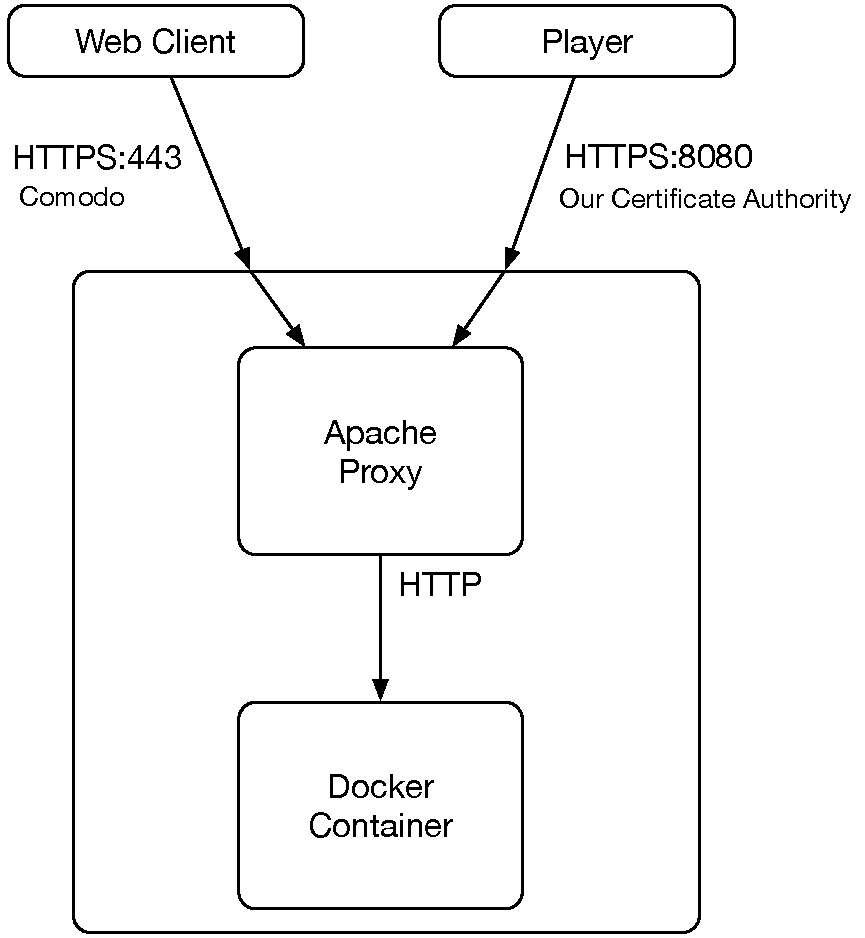
\includegraphics[width=60mm,scale=1]{docker.pdf}
 \caption{\\Arquitetura servidor e docker container}
 \label{fig:docker_c}
\end{figure}

Quando um cliente acede pelo browser ao site da loja, é-lhe fornecido um certificado assinado pela COMODO, Free SSL, que o cliente usará para navegar no site sem problemas. Este pedido, que é negociado com o Apache no servidor principal, é depois redirecionado por HTTP para o Docker container que é responsável por receber e tratar os pedidos junto com o código python (Django). Desta forma, como os pedidos apenas são tratados no container e a negociação para o HTTPS é negociada fora do container, as chaves privadas estão seguras em relação ao container.

Já quando o Player comunica com o servidor, apenas aceita pedidos do servidor que lhe apresente um certificado específico que foi anteriormente assinado pela nossa entidade certificadora criada para o efeito. Estes pedidos são depois encaminhados de igual modo para o container Docker.

\subsubsection{Utilização:}
Quando se inicia a máquina depois de fazer um "vagrant halt" deve-se executar o script "/vagrant/start-up.sh". 

\subsubsection{Comportamentos observados}
Foram realizados alguns testes com código python inserido de forma intencional no código do servidor e observou-se:

\begin{itemize}
\item Apenas tem privilégios para criar diretórios e ficheiros em pastas que pertençam ao utilizador ou grupo "www-data".
\item Não tem acesso as chaves privadas usadas para o HTTPS
\item Tem acesso à chave do Player e a todas as chaves públicas de cada device
\item Consegue ver e listar os diretórios do docker container
\item Consegue aceder à base de dados
\end{itemize}

\subsubsection{Proibição de determinados URL no Apache}

Foi tida em conta a preocupação para que o utilizador apenas conseguisse usar os endpoints para o Player na porta destinada isso, a porta 8080, para isso foi criada uma regra na porta 443 para que pedidos para os endpoints que são utilizados pelo Player fossem descartados e não fosse feito o forward para o Docker container.

\begin{figure}[!htb]
\center
 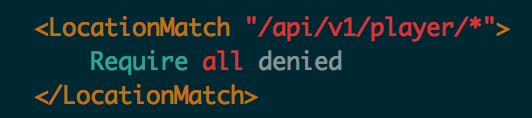
\includegraphics[width=60mm,scale=1]{player_denied.png}
 \caption{\\Proibição de acesso a endpoints do player na porta 443}
 \label{fig:docker_c}
\end{figure}

\subsubsection{Acesso ao container Docker apenas de dentro do servidor}

Para apenas permitir o acesso de dentro do servidor principal ao Docker (para fazer o forward dos pedidos HTTP) usou-se as iptables do Ubuntu para fazer deny a todos os pedidos para a porta 8002. No entanto, como estamos a usar um "Host-only adapter" o IP que o host da máquina virtual tem é o mesmo da máquina e impossibilitou que fosse testado de maneira simples.
\shellcmd{iptables -I FORWARD  --dport 8002 -j DROP}
\shellcmd{iptables -I DOCKER -p tcp --dport 8002 -j DROP}
\shellcmd{iptables -I INPUT -p tcp --dport 8002 -j DROP}

\section{Autenticação do Player junto do Servidor}

\subsection{Jar sign}
RODRIGO AQUI

\subsection{Certificados assinados pela CA do IEDCS}
Apesar das sucessivas tentativas que foram feitas para que 

\subsection{Autenticação usando o Cartão de Cidadão}

\newpage
\section{Conclusão}

Esta conclusão não é uma conclusão final, pois este projeto será realizado em duas partes.
Sendo assim vai-se optar por nesta conclusão dizer principalmente as implementações futuras e problemas encontrados.

O principal problema encontrado, foi fazer a decifra no lado do Java, depois de a cifra estar feita do lado do Python, pois muitas tecnologias disponibilizadas por este não estão disponíveis diretamente no Java, o que nos obriga a utilizar bibliotecas externas o que nem sempre é bom, pois pode-se estar a acrescentar problemas ao sistema. 

As implementações futuras que não se conseguiu implementar a tempo nesta fase do projeto, mas que contudo poderão fazer parte da próxima são:
\begin{itemize}
\item Uma sessão única sempre o device atualiza os seus dados. Este atualiza os seus dados sempre que o utilizador efetua um inicio de sessão, tenta ler um livro e muda de página. Esta solução faria com que a cifra do conteúdo do livro apenas fosse válida durante a sessão, pois assim que fosse efetuado um outro challenge com o servidor a sessão iria mudar e o Player não iria conseguir fazer a decifra.
\item A solução apresentada acima, obriga a que seja feita a cifra página a página, consoante a sessão do Player, Device e utilizador.
\item Outra ideia que nos surgiu, foi apresentar ao utilizador as duas páginas iniciais de cada EBook (Sample) de forma gratuita.
\end{itemize}

\renewcommand{\bibname}{Referências}

\begin{thebibliography}{} 
	\bibitem{Zuquete} André Zúquete, \textit{Segurança em Redes Informáticas}, 4ª Edição Aumentada, FCA - Editora de Informática, Lda.
	\bibitem{stack} \url{http://stackoverflow.com/}
	\bibitem{oracle} Java Cryptography Extension (JCE) Unlimited Strength Jurisdiction Policy \url{http://www.oracle.com/technetwork/java/javase/downloads/jce8-download-2133166.html}
	\bibitem{sigar} \url{https://support.hyperic.com/display/SIGAR/Home}
	\bibitem{SSL} \url{https://www.digitalocean.com/community/tutorials/how-to-create-a-ssl-certificate-on-apache-for-ubuntu-14-04}
	\bibitem{vagrant} \url{http://www.vagrantcloud.com}
	\bibitem{apache} \url{https://hc.apache.org/}
	\bibitem{rfc} PKCS {\#}5 e AES para a implementação em Python \url{https://tools.ietf.org/html/rfc2898}
\end{thebibliography}

\end{document}